\documentclass[procedia]{easychair}
%\documentclass[debug]{easychair}
%\documentclass[verbose]{easychair}
%\documentclass[notimes]{easychair}
%\documentclass[withtimes]{easychair}
%\documentclass[a4paper]{easychair}
%\documentclass[letterpaper]{easychair}

% This provides the \BibTeX macro
%\usepackage{doc}
%\usepackage{makeidx}
\usepackage{graphicx}
%\usepackage{epsfig}
\usepackage{url}

\def\procediaConference{Biologically Inspired Cognitive Architectures (BICA 2015)}

\title{An integrative approach to computational modeling}

\titlerunning{An integrative approach to computational modeling}

%\author{Max Talanov\\
%Kazan Federal University\\ Russia\\
%max.talanov@gmail.com\\
%\and
%Jordi Vallverd{\'u}\\
%Universitat Aut{\`i}noma de Barcelona\\ Catalonia\\
%jordi.vallverdu@uab.cat\\
%\and
%Manuel Mazzara\\
%Innopolis University\\ Russia\\
%m.mazzara@innopolis.ru\\
%\and
%Salvatore Distefano\\
%Politecnico di Milano\\ Italy\\
%salvatore.distefano@polimi.it\\

\author{
Jordi Vallverd{\'u} \inst{1}
\and
Max Talanov \inst{2}
\and
Salvatore Distefano \inst{2, 3}
\and
Manuel Mazzara \inst{4}
\and
Michael W. Bridges \inst{5}
}

\institute{
Universitat Aut{\`o}noma de Barcelona, Catalonia, Spain.
\and
Kazan Federal University, Russia.
\and
Politecnico di Milano, Italy.
\and
Innopolis University, Russia.
\and
iCarnegie Global Learning, USA.
\and
}

\authorrunning{J. Vallverdu, M. Talanov, S. Distefano, M. Mazzara, \ldots}

\begin{document}
\maketitle

\begin{abstract}
This paper provides a new cognitive meta-architecture for artificial
intelligent systems (AI and robotics). Three basic domains are the backbone 
of this architecture: physiology, psychology and philosophy, respectively 
describing sensorimotor/physical, data processing and symbolic and meta levels.
This architecture is inspired by real anthropocentric performances, and makes 
possible model from sensorimotor processes to symbolic.
\end{abstract}

\keywords{Physiology, Psychology, Philosophy, Neuroscience, Cognitive Science, Cognitive Architecture}

\section{Introduction}\label{introductionbackground}

The current literature shows several computational approaches for reimplementing human phenomena like emotions, consciousness, learning, anticipation, intuition and creativity The interest reader can find more information in \cite{neucogar2015, evaluatingcomutationalmodel, computationalmodelsemotionscognition, computationalmodelsemotion}. Often these approaches require competences in disciplines like neuroscience, psychology and philosophy that are rarely seen in software engineering teams. 

Most of this solutions produces systems with high level of concurrency and no realistic implementation of neural activity. They just attempt to mimic the effect of external stimuli.
Regarding emotions a similar approach could be followed, consisting in hardcoding the visible reaction abstracting over any neural and cognitive activity. This behavior is am effective representation of how things work at the psychological level, but cannot be mapped into lower lever models therefore missing specific details.

These solutions are too fragile, since with hardcoding we just implement reactive behavior and, for example, ignore our daily proactive behavior, i.e. our ability to learn and override direct stiumuli from the environment. This is the subject of century of western and easter philosopy.

More robust solution imply self adaptation,self learning and homeostasis maintenance. To reach such a level of flexibility and complexity we cannot ignore lower level electrochemical activity.
This approach is depicted in Figure 1 and has been introduced in \cite{p3_model}.
 
%In \cite{senticcomputing} a direct approach is implemented, with the disadvantage 
%of requiring limited reference to the actual neuronal computations of the human brain. 
%An more realistic alternative way could be to move all the details of different 
%perspectives into the model and to use a bottom up approach to implement the system 
%building, increasing the complexity from cellular level to upper abstractions of the
%philosophical perspective. This approach is depicted in Figure 1 and was
%introduced in \cite{p3_model}.

\begin{figure}[htbp]
\centering

\includegraphics[width=0.9\textwidth]{layers_binding}
\caption{Figure 1. Domains binding}
\end{figure}

An anthropocentric-inspired model has to take into account three
activity layers (that we will call \textit{domains}): 

\begin{enumerate}
	\item Physiological
	\item Psychological
	\item Philosophical
	
\end{enumerate}

%with them it is possible to build an uniform approach for
the complete description of an object of research. 

A robust computational system should be implemented via low-level
constructs like artificial neurons or other basic cognitive bricks. 
This could make it easier to make a scalable system from scratch to high
cognitive processes. This approach, in turn, raises several questions,
such as ``what are those domains in computational systems that
correspond to physiology, psychology, philosophy?'', ``how those domains
are related to each other?'', ``how are those new domain related to
current cognitive architectures provided by computer sciences?'', ``what
is the exact nature of the domains-phenomena which we suggest to
recreate in the computational system?'' or ``are those new domains
strictly necessary? and why?''

We try to provide answers to these questions, recognizing that this
could be just a starting point in a discussion, but not an exhaustive
explanation. In the section ``Cognitive Science'' we introduce the
overall picture of the anthropocentric domains: philosophy, psychology,
physiology. In the section ``New Domains Definitions'' we introduce
three new domains that are brought to reality by several attempts to
understand the structure of possible views on reproduction of human
phenomena and mechanisms in a computational system and the approach to
organize the concepts of the views. In the section ``Justification'' we
try to answer the question - ``What is the motivation to create these
domains?''. We also draw examples of future possible applications in
section ``Future Possible Applications''.

\section{Cognitive Science}\label{cognitive-science}

\subsection{Overall Picture}\label{overall-picture}

Natural cognitive systems are not just the sum of different specialized
modules. Most recent research has shown how the body, the mind and some
extended related varieties (symbolic tools, cognitive extensions,
ecological conditions,\ldots{}) are work in parallel following a
continuous interaction. Sensorimotor processes are influenced by
emotional memories that orient attention scope, task-planning or even
internal simulation mechanisms \cite{ferraz2009}. According to new ideas
on grounded cognition (which includes notions like embodied, extended,
situated or enactive cognition), a cognitive process is the result of
coordination among several domains. We have discretized them following a
tripartite model: physiology, psychology, and philosophy. We are neither
abandoning nor neglecting the role of socio-cultural variables (they can
be added or created later), but we consider that from a functional
perspective, these three domains capture the basis of cognitive
activity.

Our attempt is related but not reducible to the `cognitive hexagon'
model widely known in cognitive sciences \cite{miller2003}. It
illustrates the fields that contributed to the birth of cognitive
science, including linguistics, neuroscience, artificial intelligence,
philosophy, anthropology, and psychology. Our model takes into account
only three functional activities that define a cognitive process from a
broadly understood bodily perspective. From a formal perspective
Philosophy, Anthropology and Linguistics are different instantiations of
symbolic processes (individual or social ones). In this sense our domain
called `philosophy' is not equivalent to the historical domain of
Philosophy, but works on how a system creates symbolic semantic and
syntactic values or strategies. And from a bodily perspective,
Neuroscience is embedded into our physiological domain.

We assume at the same time that the ways we process information at
psychological and philosophical levels are influenced following a broad
range of distributions of socio-cultural variables, but in any case they
are not part of the cognitive mechanism. The symbolic and cultural
values are added by a social training process that can be partially
reproduced (think for example of Luc Steel's Language Games
\cite{steels}, if we consider robot-robot learning processes; on in HRI
supervised training) or can be directly programmed into artificial
cognitive memories.

\subsection{Relations of the Domains}\label{relations-of-the-domains}

\begin{figure}[htbp]
\centering

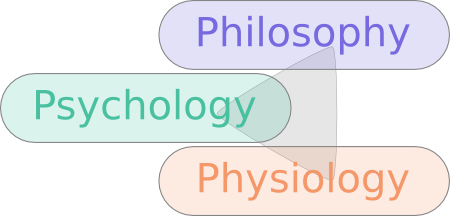
\includegraphics[width=0.4\textwidth]{cognitive_triangle}
\caption{Cognitive triangle }
\end{figure}

Our model runs perpetual loops among all the domains, without a
central-control structure, despite the crucial role of the philosophical
level (where we could place the `artificial consciousness'). Obviously,
from a systemic perspective, it is a layered model, but the interactions
are open among these levels.

Even considering the superstructure of `consciousness', regarding it as
an integrative control system, the rest of systems work in parallel
solving problems at several levels. It is the same way as human brain
activity: running bodily, sensorimotor, simulating processes beyond any
conscious control. At the same time, it emulates the intentional nature
of human brains, always processing information according to pre-wired
structural necessities based on morphological constraints. The only
difference between our model and a natural being with a similar one is
that the intentionality that guides the system is pre-programmed by us
instead of being the result of evolutionary forces.

\section{New Domains Definitions}\label{new-domains-definitions}

\begin{figure}[htbp]
\centering

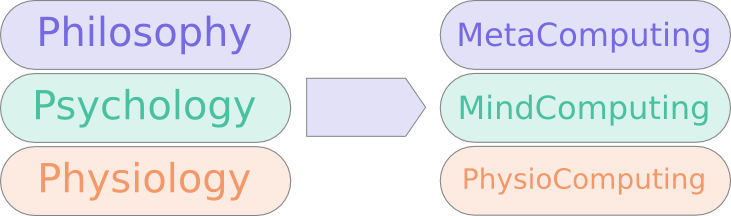
\includegraphics[width=0.9\textwidth]{p3_model}
\caption{Domains mapping}
\end{figure}

Each of three domains is made of basic elements, which we call
``bricks'', and consider them functional units that solve system
necessities or strategies.

From a physiological perspective, the body is built by materials that
shape it, as well as sensors that provide information which will be
processed by the brain; here, neuroscience provides us with a very basic
``brick'' of the brain, the neuron, that actually is used as main
inspiration for artificial neural networks. This living cell has an
option to reorganize its connectivity hence affecting the properties of
the neural network without any external intervention. A computational
system in order to progress should have living cell properties of
reorganization.

From neurophysiological basis emerge cognitive programs that solve
adaptive problems\cite{cosmides}. Think for example on navigation,
mating, vision, emotional management, attention or language
processing/expression, among a myriad of possible modules. Our brains
evolved for millions of years to produce behavior and more specifically,
social behavior.

We should also make a distinction between pre-symbolic and post-symbolic
contexts in human cognitive processes, because the impact of the later
changed completely the environment and survival strategies of humans. It
is also much easier to deal with pre-symbolic brain architecture in
order to isolate the basic units of psychological activity.

So, from the perspective of psychology \cite{primer_affect_psychology,
tomkins} there are several phenomena like emotions that are grounded
in neurobiological basement of neuromodulation \cite{duchaine,
natureofemotions, cubeofemotions} and could have significant impact on
the computational system especially a neurobiologically inspired one
\cite{affective_computing_book,computational_emotional_thinking,computationalmodelsemotion}.
Emotional states influence decision making \cite{paulus2012},
motivation, learning, subjective experience, thinking
\cite{whatdoesitmeanforcomputer} in real time systems that are crucial
for social collaborative computational systems.

From the philosophical perspective \cite{emotionmachine} there are
several models of consciousness that could be recreated in computational
systems. Establishing a cross-disciplinary approach of recreating from
the basic constructs to the top-level concepts we could get to the point
of the emergence of important phenomena like consciousness,
understanding or thinking. At a theoretical level we can easily identify
the bricks of philosophical performing, and they follow two different
spheres: a) semantics: basic memes that are considered axioms of the
reasoning process, such as god, soul,truth, reason, meaning, evidence,
demonstration, cause, etc.; and b)syntax: the rules and strategies
considered as good ones to produce good knowledge, that is: syllogistic,
monotonic logic, non-monotonic logic, abduction, induction, deduction,
simulations, emulation, heuristics, hermeneutics, common-sense (tacit
knowledge), and so on.

\subsection{Integrative approach}\label{integrative-approach}

Current cross disciplinary approaches direct us to the
cross-disciplinary models that should take into account several domains.
There is one more aspect of this distribution of models focus: as the
result we should build the models that take into account concepts of
different scales, constructing from the basic blocks of networks, with
other complex structures emerging to support higher level phenomena. But
from the other side we should use overall meta-pictures of complex
phenomena like: consciousness, thinking, or cognition.

Imagine a life of a single living neuron: it creates synapses, fires
spikes, deletes synapses, dies (while even some others are born)
\ldots{} Then imagine the life of a cortical column: approximately
10,000 cells that implements some basic cognitive functions like
horizontal line recognition: Going one step further, we reach a bigger
area like visual cortex, where interconnected columns get synchronized.
At this level of granularity more generic phenomena like neuromodulation
comes on stage implementing emotions here the connection to
psychological and philosophical phenomena domain emerges. From the
meta-perspective, such models of mental activities like ``Model of six''
\cite{emotionmachine} and ``H-CogAff'' \cite{sloman2003} provides us
with the overall map to fit with low level concepts in gaining proper
low level neuronal computational basis. This holistic (meta) and
functional integrative approach that we call ``ubique'' provide us the
benefits of both overall picture and understanding of actual
computational neuronal mechanisms.

\subsection{Artificial living systems}\label{artificial-living-systems}

Most of AI architectures have been following ideas derived from Von
Neumann architectures instead of using the available information of
living entities \cite{brooks2}. This has made more difficult to merge AI
with artificial life (Alife) researches, at least from a naturalistic
perspective \cite{alife}. The force that guide our approach is how to
implement into AI bottom-up and socio-biologically inspired
architectures.

There are several constructs that we introduce to build a proper
foundation of new domains. From our perspective, the most basic building
``brick'' is the artificial living cell (ALC), which performs 2 main
functions: reproduction and feeding. There are two consequences to the
reproduction function of ALCs in a computational systems domain. The
first is the regeneration of computational and/or robotics systems. The
second is the ability of an artificial neuronal network (brain) to
self-organize/self-optimize to potentially produce emotions and
motivation, common sense logic, memory, consciousness (e.g., awareness,
learning, anticipation, subjective experience), intuition, perception
and understanding, creativity, or dreaming/sleep. On the other hand the
basic ``bricks'' via artificial living neuronal network creates proper
environment for the MindComputing phenomena creation and development.
The functions can be accelerated by artificial evolution or directly
implemented as some form of interest according to the chosen functional
purposes. Therefore, we are suggesting the design of Alife
self-organizative architectures that can be controlled computationally.

\subsection{PhysioComputing}\label{physiocomputing}

PhysioComputing implements the \emph{physiology of computing}. It is the
scientific study of the hardware and software implementing intelligent
systems/approaches that are capable of executing the set of phenomena
listed above ALS with basic ``block'' of ALC. It should take into
account implementation details like distributed computing systems or
supercomputer systems and cellular analogies with human organism of
vital functions, life and existence in the ever-changing natural
environment. The scope of PhysioComputing is to provide structural,
functional, devices-embedded, distributed, communicational aspects of
the implemented systems in a devices, chips, antennas, engines etc. with
a software that creates proper collaboration among cognitive operations.

\subsection{MindComputing}\label{mindcomputing}

MindComputing is the \emph{psychology of computing} and is an academic
study of phenomena of ALS that implements main components of the
artificial intelligent systems analogous to natural intelligent systems
like mind. It should consider the high level details of phenomena taking
into account broader and more conceptual approaches of the artificial
mind operation based on the concepts/views/theories/hypotheses
introduced in the PhysioComputing. The scope of the MindComputing is to
reproduce the important cognitive functions of ALS, those that also make
possible social collaborations as well as generate behavior for
artificial individuals.

\subsection{MetaComputing}\label{metacomputing}

MetaComputing is the \emph{philosophy of computing}. MetaComputing is
the study of fundamental problems of an ALS. It should use several views
possibly based on the MindComputing and PhysioComputing concepts, and
could be an integral part of the philosophy. The creative ways of
obtaining new knowledge (this includes information management,
strategies, ways to obtain raw data) are considered on this level. As
humans work inductively, abductively or statistically, improvising in
different moments and situations: this implies the necessity of the
exploration of cognitive-knowledge meta-levels. The scope of
MetaComputing includes definitions and high-level views on the problems
of ALS (organisms), artificial individuals/personalities as part and
extending the Artificial Intelligent domains. In other words,
MetaComputing represents a methodological challenge that could be solved
thanks to emotional cognitive architectures.

\subsection{Relationships}\label{relationships}

Although there are specific domains to each level, we could consider
cognition as a bodily grounded experience. Recent neuroscientific
researches provide evidence that sensorimotor processes are at the core
of the brain processing,thus metalevels cannot be completely free from
physical constraints.

In our model the three domains are deeply interconnected.The dynamical
and tridimensional activities of our model must be clarified:
highlighting both horizontal and vertical relationships among our
domains will allow the emergence of different interpretations. For
example, any block (PhisioComputing, MindComputig, MetaComputing) is
independent, and therefore independently mapped into the application
domain, or as a whole. At the same time layers are connected and
interdependent in a layered way, as well as complex functions at higher
layer are based on simpler ones provided at lower layer(s).

\section{Justification}\label{justification}

In our days, AI or robotic cognitive requirements have been based on
well-defined mind processing emulations, or even to very narrow aspects
of expert symbolic processing, achieving impressive results. But no
research has provided a structure to integrate parallel and
interconnected levels of functioning. There are several reasons: the
complexity of the system, the necessity of bigger computing power or the
lack of confidence into Bayesian statistics (the closest to natural
neuron activities), but above all there is the intellectual necessity of
control. Computational approachesto autonomous systems are engineered,
modeled, and look to satisfy functional necessities with small losses,
minimizing blind changes and maximizing efficiency and profit.

Instead of putting a whole human being in the center of study we propose
to focus on an artificial living system or an artificial organism and
develop scientific domains around this phenomena. From this perspective
during the development of AI systems we use only one level of
abstraction that is effectively implemented in the computational system
or literally in the code. Approaches like this usually miss either
low-level details in case of direct implementation of the psychological
models and thus don't really work like human body works, or lacks the
references to high-level phenomena like emotions (which are at the same
time low-level information selecting/modulating mechanisms). We could
refer to works of Marvin Minsky \cite{minsky1988, emotionmachine} and
Aaron Sloman \cite{sloman2003} that incorporate this trifocal view on
the problems like consciousness or thinking.

In the pursuit of the emulation of the basic properties of human beings
(intelligence, creativity, attention, and so on) several attempts have
been made, parsing the complex behavior of human mind into ``feasible''
expert domains.

Once some small successes have been achieved, the necessity of increased
performance of these artificial cognitive systems has faced researchers
with a hard problem: how to make a system that integrates dynamic,
multidimensional and scarce data, all of them present in decision-making
processes in open environments. The general trend has been to turn the
interest from the mind, as the first symbolic AI approaches did, to the
grounded cognitive paradigms \cite{Barsalou2008}.

In a nutshell, a holistic view about the human body and their multilevel
cognitive processes (sensorimotor, social, emotional, symbolic) has been
increasingly implemented. But none of the previous models have
considered this process as a necessary and unified project; our ubique
(holistic and functional) model suggests this for the first time,
establishing clear functional correlation among activity domains. This
makes it possible to understand how to approach artificial emotions or
even artificial consciousness. For functional purposes, we've selected
three domains that make this analysis possible.

\subsection{Morphological}\label{morphological}

Morphology is the basis of the whole system, and it is never neutral: it
is oriented to some specific actions. Our model is a simplified but
powerful way to design computational layers of action. It is not a
simple new subsumption architecture, but an integrated way to understand
a cognitive system. Obviously, it has a subsumption architecture, but
this doesn't explain its whole dynamics. It is not a question of some
specific terms or classifications, it is a question about a research
approach. The complexity of the consciousness problem demands the use of
an ubique approach: literally take in account low-level and high-level
details in one model. Our trifocal ubique approach is considered to
provide benefits of both functional and holistic approaches in one
model, this way all the complexity is concentrated in the theoretical
model not in the implementation programmatic or robotic.

\subsection{Technological}\label{technological}

The neurobiologically inspired revolution that is going at the current
moment demands new technologies starting from the base of transistors
and integrated circuits \cite{neurocomputing}. Current hardware
architectures are not effective to satisfy today requirements: to
simulate 1\% of human brain RIKEN specialists used 250 supercomputers
`K'\cite{RIKEN}. At the same time new perspectives to use computational
power compared to human brain draws new demands of the hardware-software
architecture of new computational systems that would be capable of:
everyday-life decision making in real time, social communications and
collaborations, consciousness, human-like thinking, understanding of
humans and their life problems to be effective in collaborations with
people and capable of helping solving complex problems of nearest
future.

There is a very important technical point that we also solve with our
model: the statistical mind. Most uses of statistical techniques in AI
are implemented following a symbolic approach. With a grounded vision of
a cognitive process, we would be able to design Bayesian-inspired
techniques that emerge from a cooperation between domains, basically
from sensorimotor coordination. This adds a more natural way of
embodying natural calculations, following a modal perception and
integration model, although our system can implement any amodal-working
method shown as robust and reliable enough. We show the path towards a
real mixture of modal and amodal sets of data performed interactively by
our three domains.

\subsection{Philosophical}\label{philosophical}

At this point it seems reasonable to ask ourselves if there is a
philosophical foundation for the three new domains. The answer is
positive. For several reasons. Originally in Eastern as well as in
Western traditions humans were considered as the sum of mind and body
\cite{dualism}. This allowed the emergence of a mechanistic view of body
and also to the metaphors of the human as a machine with separate
functional modules, and later it inspired computers designs (following
Von Neumann arquitectures). But with the advances of cognitive sciences,
specially thanks to neurology, this dualism was broken and the notions
of grounded, embedded, situated or extended cognition emerged. With
these advances, became obvious that despite the existence of different
functional layers, an organism behaves as a whole, integrating parallel
processes that are initially focused into different specialized tasks or
functional domains. Thus, we can talk about a \textbf{systems cognition
model}, an idea we've created in order to answer to the real properties
of cognitive events. Here, several functional layers can be identified
at the same time that the continuous interaction of these layers is
respected by this ubique (holistic and functional bottom up)approach.
Human brains and bodies are performing several connected but at the same
time separated cognitive processes (body regulation, sensorimotor
evaluation, outputs simulation, emotional managing, task planning,
\ldots{}). Our model allows to discretize and to merge at the same time
these three basic perspectives of cognitive managing.

\section{Future Possible
Applications}\label{future-possible-applications}

Our model is ubique: holistic as well as functional bottom up approach
that could help to design robots with a global functional identity.
Robots with integrated functionalities thought from scratch are more
efficient thanks to the necessity of the elements that integrate the
system. At the same time, it could help to create of less predictable
but more rich behaviors. It is reinforced by the social nature of our
architecture. A ``cognitive'' is a being that tries to survive reacting
to the environments and other living entities. It is true even at the
basic level of bacterial communication and cooperation. Our trifocal
approach could make it easier to design robots with specific and unique
characters or moods. This could help to achieve innovative ways of
dealing with new psychological problem of robots.

\section{Conclusion}\label{conclusion}

The new wave into AI architectures will surely come thanks to the
implementation of biologically inspired architectures. This is a
generally accepted view among the community (emotional architectures,
neuromorphic chips, emotional NN, neuromodelling,\ldots{}). But at the
same time, the psychological and naturally generated symbolic levels
have still not been added to these architectures. Despite the existence
of swarm robotics or even social robotics and affective computer
advances, no similar architecture has been provided until now. We
provide an ubique: integrative, modular, dynamic and decentralized
cognitive architecture that solves several requirements from the complex
necessities of contemporary AI and robotics.

\section{Acknowledgment}\label{acknowledgment}

We thank Dr.~Marat Minlebaev and Alexander Tchitchigin for the critical
reading and useful comments.

\bibliographystyle{plain}
\bibliography{domains_intro}
\end{document}